\section{Search in the Same-sign Dilepton Final State}
\label{sec:ss}

This section presents a search in the same-sign (SS) dilepton final state, based on 10.5 fb$^{-1}$.
A wide variety of new physics processes may produce events with SS leptons, which provide a very clean
final state due to low SM background expectations. In particular, this final state is sensitive to 
direct pair production of bottom squarks with $\tilde{b}\to t \chi^{\pm}\to t W \lsp$ depicted in Fig.~\ref{fig:diagrams}(d),
as well as to gluino-mediated production of top and bottom squarks.

We select events with two leptons (e or $\mu$) with \pt\ $>$ 20 GeV and dilepton invariant mass $m_{\ell\ell}>8$ GeV. 
We reject events with a third lepton with \pt\ $>$ 10 GeV that forms an opposite-sign
same-flavor pair with $76 < m_{\ell\ell} < 106$ GeV with either selected lepton, to suppress
the background from WZ and ZZ. We require the presence of at least two jets with \pt\ $>$ 40 GeV.

This analysis is an extension of a previous search in the same-sign dilepton final state~\cite{ref:ss_inclusive}.
In that analysis, the background is dominated by \ttljets\ where one lepton is from the W decay and the other
lepton is produced in the decay of one of the b-jets. In this analysis we require the presence of at least two
b-tagged jets (using CSVM). The requirement that both b-jets are identified and well-separated from the selected leptons
reduces the \ttljets\ background by an order of magnitude. 

There are three sources of SM background passing the above preselection. 
The first background source is referred to as ``fake leptons'' and includes leptons from heavy-flavor decay, 
misidentified hadrons, muons from meson decay in flight, or electrons from unidentified photon conversions. 
This background is estimated from a sample of events with at least one lepton that passes a loose selection 
but fails the full analysis identification and isolation requirements. This sample is weighted by the probability 
for a fake lepton satisfying the loose selection to also pass the analysis selection, which is determined based 
on studies of fake 
leptons in jet events. The second background, estimated from MC, consists of rare SM processes and is dominated 
by $t\bar{t}$W and $t\bar{t}$Z. The systematic uncertainty on both the fake lepton and rare backgrounds is 50\%. 
A third, small background contributions is from ``charge flips'' and consists of events with opposite-sign leptons 
where one of the leptons is an electron whose charge is misreconstructed. This background is based on MC predictions,
which are validated using a sample of Z$\to e^+e^-$ events.

Signal regions are defined by placing additional requirements on the jet multiplicity, b-tagged jet multiplicity, 
\met, and $H_T$, defined as the scalar sum of the transverse momenta of selected jets. The observed data yields 
in these signal regions are compared to the SM background expectations in 
Table~\ref{tab:ss}. Good agreement is observed between the data and the expected background in all signal regions.

In Fig.~\ref{fig:ss_interpretation}(a),tThe results are interpreted using the model of bottom squark pair 
production with $\tilde{b}\to t \chi^{\pm}$ depicted in Fig.~\ref{fig:diagrams}(d).
The most sensitive signal region in most of the model parameter space is SR3 (see Table~\ref{tab:ss}).
These results probe bottom squarks with masses up to 450 GeV.
The constraint on the bottom squark mass from naturalness is similar to that on the top squark, requiring 
a mass less than 500-700~GeV. Several additional interpretations for models with gluino-mediated top and 
bottom squark production are presented in Ref.~\cite{ref:ss}.


%\begin{table}
%\centering
%\caption{Please write your table caption here}
%\label{tab-1}       % Give a unique label
%% For LaTeX tables you can use
%\begin{tabular}{lll}
%\hline
%first & second & third  \\\hline
%number & number & number \\
%number & number & number \\\hline
%\end{tabular}
%% Or use
%\vspace*{5cm}  % with the correct table height
%\end{table}


\begin{table*}[t]
\centering
  \caption{\label{tab:ss} Summary of the results of the search in the same-sign dilepton final state.
    Several signal regions (SR) are indicated, including the kinematic requirements, the prediction of the three background (BG) contributions,
    the total background, and the observed yield in data. The jet multiplicity requirement in the first row includes both b-tagged and untagged jets. The uncertainty includes the statistical and systematic components.}
  \tabcolsep 2.7pt
  \begin{scriptsize}
    \begin{tabular}{l|c|c|c|c|c|c|c|c|c}
\hline
\hline
& SR0 & SR1 & SR2 & SR3 & SR4 & SR5 & SR6 & SR7 & SR8 \\
      \hline
      No. of jets            & $\geq 2$               & $\geq 2$               & $\geq 2$               & $\geq 4$               & $\geq 4$               & $\geq 4$               & $\geq 4$               & $\geq 3$               & $\geq 4$       \\
      No. of btags           & $\geq 2$               & $\geq 2$               & $\geq 2$               & $\geq 2$               & $\geq 2$               & $\geq 2$               & $\geq 2$               & $\geq 3$               & $\geq 2$       \\
      Lepton charges         & $++/--$                & $++/--$                & $++$                   & $++/--$                & $++/--$                & $++/--$                & $++/--$                & $++/--$                & $++/--$        \\
      \met                 & $> 0$ GeV             & $> 30$ GeV            & $> 30$ GeV            & $> 120$ GeV           & $> 50$ GeV            & $> 50$ GeV            & $> 120$ GeV           & $> 50$ GeV            & $> 0$ GeV     \\
      $H_T$                  & $> 80$ GeV            & $> 80$ GeV            & $> 80$ GeV            & $> 200$ GeV           & $> 200$ GeV           & $> 320$ GeV           & $> 320$ GeV           & $> 200$ GeV           & $> 320$ GeV   \\
      \hline
      Charge-flip BG         & $3.35 \pm 0.67$ & $2.70 \pm 0.54$ & $1.35 \pm 0.27$ & $0.04 \pm 0.01$ & $0.21 \pm 0.05$ & $0.14 \pm 0.03$ & $0.04 \pm 0.01$ & $0.03 \pm 0.01$ & $0.21 \pm 0.05$\\
      Fake BG                & $24.77 \pm 12.62$ & $19.18 \pm 9.83$ & $9.59 \pm 5.02$ & $0.99 \pm 0.69$ & $4.51 \pm 2.85$ & $2.88 \pm 1.69$ & $0.67 \pm 0.48$ & $0.71 \pm 0.47$ & $4.39 \pm 2.64$  \\
      Rare SM BG             & $11.75 \pm 5.89$ & $10.46 \pm 5.25$ & $6.73 \pm 3.39$ & $1.18 \pm 0.67$ & $3.35 \pm 1.84$ & $2.66 \pm 1.47$ & $1.02 \pm 0.60$ & $0.44 \pm 0.39$ & $3.50 \pm 1.92$  \\
      \hline
      Total BG               & $39.87 \pm 13.94$ & $32.34 \pm 11.16$ & $17.67 \pm 6.06$ & $2.22 \pm 0.96$ & $8.07 \pm 3.39$ & $5.67 \pm 2.24$ & $1.73 \pm 0.77$ & $1.18 \pm 0.61$ & $8.11 \pm 3.26$  \\
      Event yield            & 43                & 38                & 14                & 1                & 10                & 7                & 1                & 1                & 9              \\
      \hline
%      $N_{{UL}}$ (13\% unc.) & 27.2   &26.0   &9.9    &3.6    &10.8   &8.6    &3.6    &3.7    &9.6 \\
%      $N_{{UL}}$ (20\% unc.) & 28.2   &27.2   &10.2   &3.6    &11.2   &8.9    &3.7    &3.8    &9.9 \\
%      $N_{{UL}}$ (30\% unc.) & 30.4   &29.6   &10.7   &3.8    &12.0   &9.6    &3.9    &4.0    &10.5 \\
      \hline
    \end{tabular}
  \end{scriptsize}
\end{table*}


\begin{figure*}
\centering
%\begin{center}
\begin{tabular}{cc}
\subfloat[] {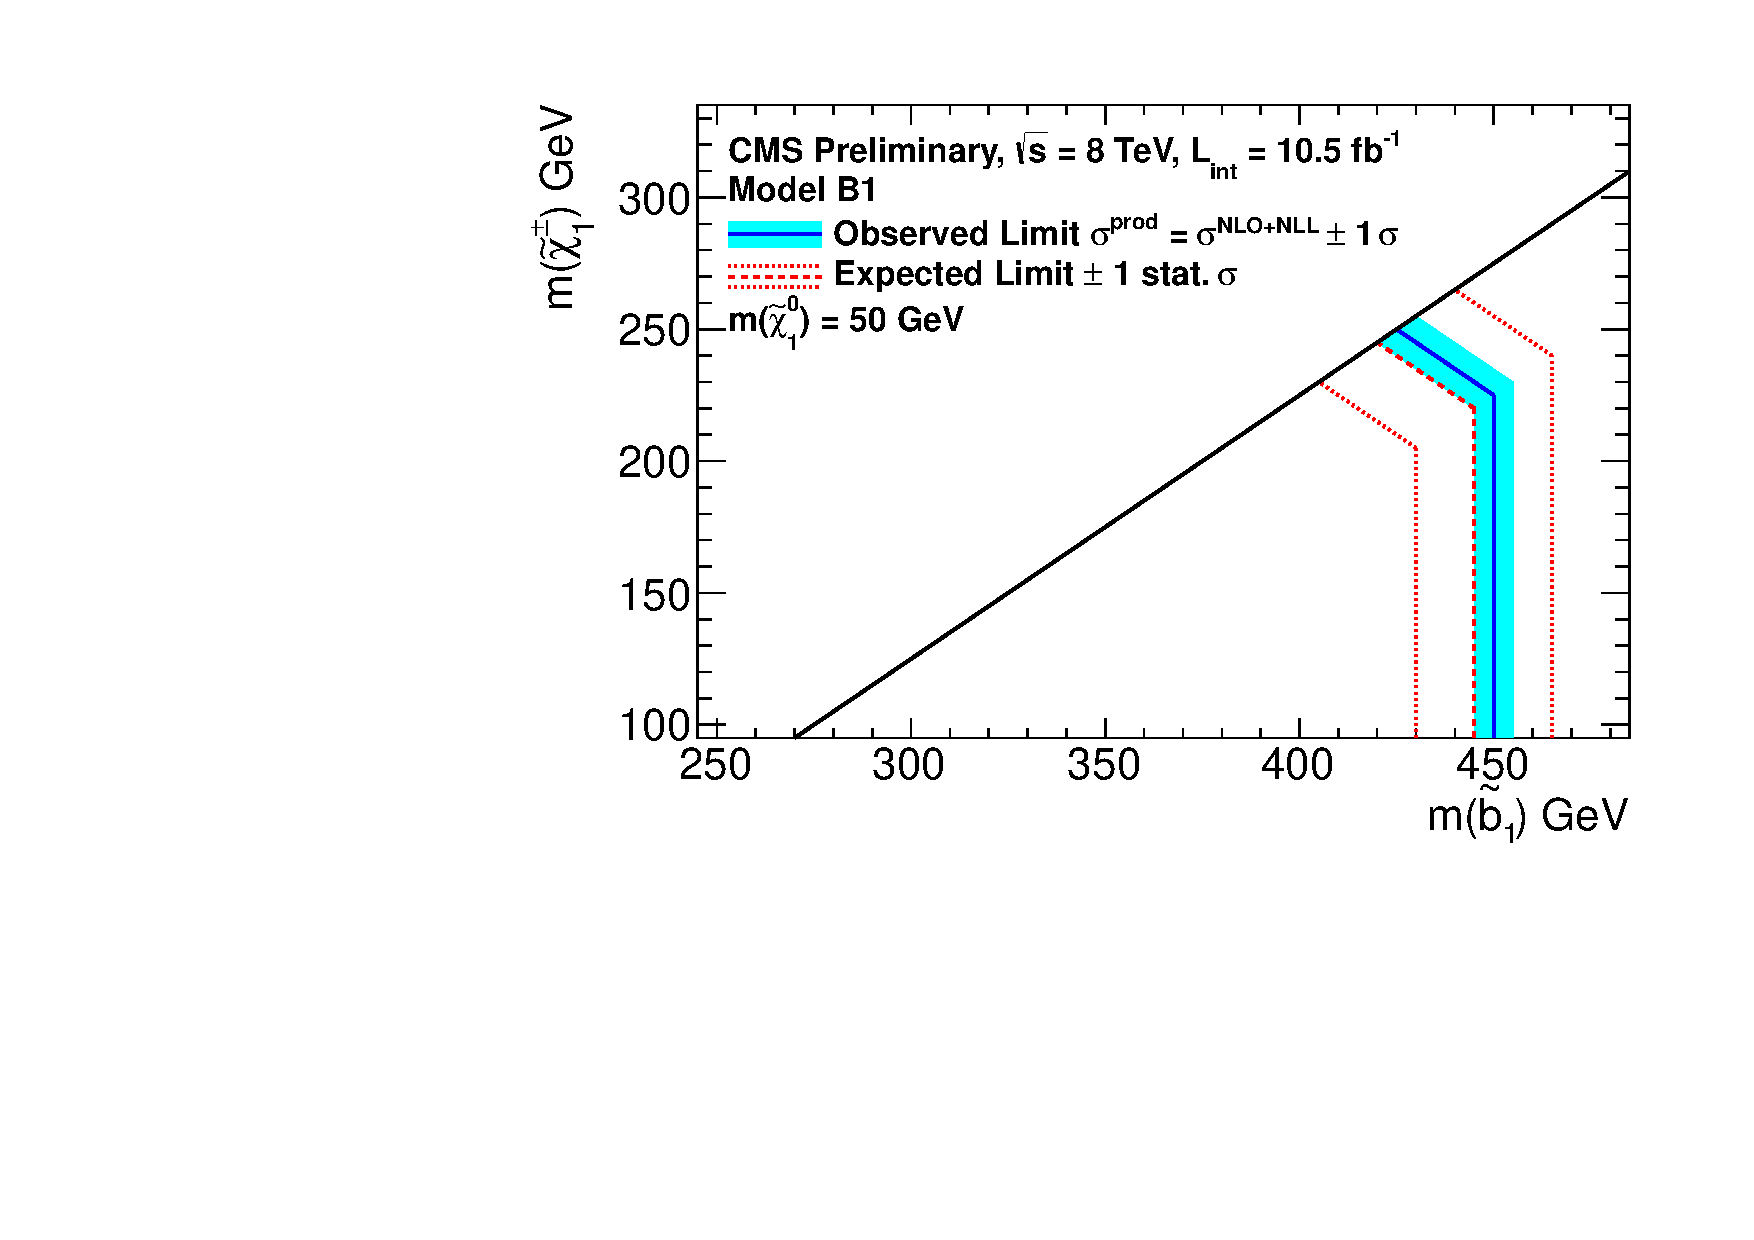
\includegraphics[width=0.5\textwidth]{HCPPlots/SS_B1.pdf}} &
\subfloat[] {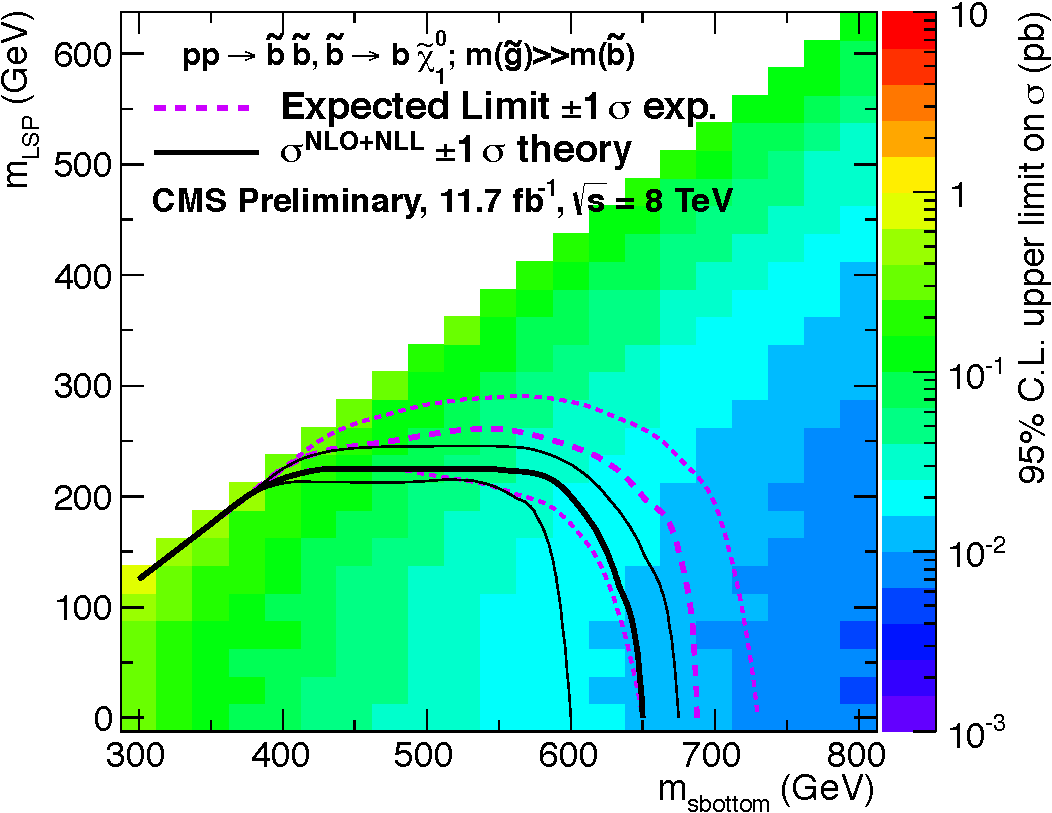
\includegraphics[width=0.4\textwidth]{HCPPlots/T2bb_interpretation.pdf}} \\
\end{tabular}
\caption{
Interpretation of the results of the search in (a) the same-sign dilepton final state for
bottom squark pair production with $\tilde{b}\to t\chip$ depicted in Fig.~\ref{fig:diagrams}(d), and (b)
the all-hadronic final state for bottom squark pair production with $\tilde{b}\to b\lsp$ depicted in Fig.~\ref{fig:diagrams}(c).
\label{fig:ss_interpretation}
}
%\end{center}
\end{figure*}

